\section{Hypothesis}
We suggest that, for on a fixed hardware platform, the total running time of a boolean
circuit follows this analytical model:
\begin{equation} \label{eq:1}
T = \max\{ t_g + t_e, t_m(w) \}
\end{equation}
where $T$ is the total elapsed (wallclock) time in processing a single gate, $t_g$
is the CPU time for generating a gate, $t_e$ is the CPU time for evaluating a gate,
and $t_m(w)$ are the memory-stalls from the gate-generation and gate-evaluation
computations.
\par
Any hardware platform evaluating an obfuscated circuit $C$ needs to represent its gates
in a readable and comprehensible internal format that is stored in memory, then apply the logical function of every
gate on the gate's relevant inputs and finally store those results in memory to be used by other gates.
The evaluation of each each gate has a time cost $t_g$ related to the creation of its
representation on the evaluation's platform, and a second time cost $t_e$ related
to the pure evaluation of the logical function of the gate.
\par
Our prediction is that $t_g$ and $t_e$ are constant or of a similar order for any gates in
any given random circuit of the same width $w$.
\par
We introduce $t_m(w)$ as the variable time component in a gate's evaluation. It
is related to the organisation of the circuit and how it is represented on a platform's
memory. It can also vary from one platform to another. But for a fixed platform, we predict that it is a function of the width $w$.
If the width $w$ is wider than the last level of cache of CPU of the hardware platform
evaluating the obfuscated circuit under test, then we are most likely to experience
memory stalls that severely affect performance. In that scenario, the evaluation time
is dominated by the time the CPU spends fetching the inputs of a gate, as opposed
to the time it requires to evaluate the gate's logical function, once the inputs are
available. This would confirm that the overhead introduced by obfuscation makes obfuscated
program unadapted to current hardware and therefore inefficient for end users.
\par
If the proposed analytical model is validated by our results, we expect it to be
also valid for other platforms of a similar range.
\section{Methodology}
We now describe the algorithm used to simulate an obfuscated boolean circuit and
the tools used to measure its execution time on a hardware platform.
\subsection{BPW Generation}
Thomborson proposed a space-efficient and computationally-appropriate file format
called \textit{BPW} for the evaluation of very large Boolean functions with bounded
program widths\cite{clark}. In the \textit{BPW}, Gates of a circuit are represented
by descriptors holding information about their type (AND, OR, $\dots$) and are
sequentially encoded inside the file's body. In our experiment we generate random
boolean circuits (which evaluate random boolean functions) with varying width $w$
for a fixed circuit size $N$. The relationship between a circuit width $w$ and
depth $D$ is $ N = w \times D $, so for $ w = N$ the circuit has depth 1.
\par
The generated circuits are represented using a simplified BPW format by storing
the gate type and the input indices only and by making following assumptions about
the properties of the circuit under test.
\begin{enumerate}
\item All circuits have size $N = 10^8$
\item $w$ takes the values $\{10^3, 10^4, 10^5, 10^6, 10^7, 10^8 \}$
\item A circuit input array has size $w$.
\item Any given level $L$ has exactly $w$ gates.
\item Every gate has only one output.
\item A circuit output array has size $w$.
\item Any given gate from a level $L_i$ has between one and three inputs that come
from level $L_{i-1}$ exclusively, such that:\break $G_i = f(X)$, where $f$ is a
boolean operator and $X$ is an 8-byte array of size 1, 2 or 3.
\item The output of a gate is written inside the output array at the same index
of the gate. $G_i(X) = Output$ $array[i]$.
\end{enumerate}
The \textit{rand()} method from the \textit{C} standard library was used to
attribute a random type to a gate, as well as assign its input indices.
\par
The entire circuit is generated prior to its evaluation. The generation step
executed initially is therefore not monitored for performance. The resulting
circuit is stacked gate by gate in a simplified BPW file.
\par
Following the initial BPW format developed by Thomborson, the first 4 bytes represent
the header of the a BPW file\cite{clark}. The following bytes then represent the
total gates of the circuit. All gates are sequentially represented from index $0$
to index $10^8-1$. A given gate's encoding varies from 9 to 25 bytes. The first
byte holds the type of the gate. The following 8 to 24 bytes present the input
indices encoded over 64-bits each. The gate's representation could be optimised
to the minimum bytes needed to encode a gate. Compression could also be used to
save disk space. We chose to keep the existing model for simplicity. As mentioned
earlier, the size of the circuits under test was fixed to $N = 10^8$. We modelled
14 types of Gates; 1 $\times$ 1-input, 6 $\times$ 2-input and 7 $\times$ 3-input
gates. On average, a gate has 2.43 inputs encoded with 8 bytes per input plus
one byte for the gate type. The average size of a BPW file storing a circuit is
therefore $avg(sizeof(Gate)) * 10^8 \approx 2 GB$.


\subsection{Evaluation}
A circuit evaluation is sequential for both gates and levels. During execution,
gates of a level $L_i$ are processed in ascending order of index in the level.
Inputs indices for a gate are randomly distributed over [0, $w$-1]. Every gate
retrieves its relevant inputs as described by the gate descriptor. Once a gate is
processed, its output is stored in the output array at the same index as the gate.
Once all the gates of level $L_i$ are processed, the execution cursor moves to
level $L_{i+1}$. The hypothesis is that the random distribution of gate input
indices will significantly affect the overall performance of the circuit for
large $w$, as the entire input array cannot fit in the cache. Figure \ref{fig:level}
describes how a level is evaluated.
\begin{figure}[h!]
	\center
	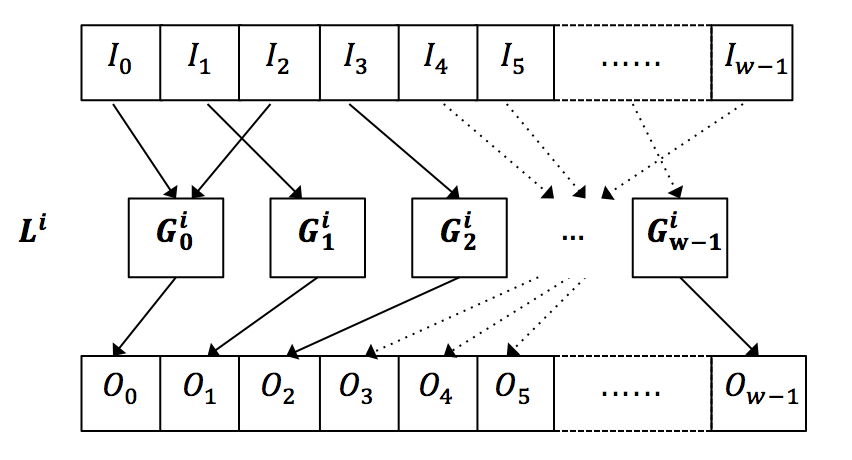
\includegraphics[width=0.8\textwidth]{img/level.png}
	\caption{Simple description of Level $L_i$ evaluation}
	\label{fig:level}
\end{figure}
\par
\subsection{Hardware}
Obfuscators might occasionally run on super computers, however it is likely that
viable commercial use of obfuscators would require them to run on mass market
platforms such as smart phones, battery powered laptops and desktop computers\cite{clark}.
The target platform for the circuits evaluation is a mid-level desktop computer.
The CPU is a 64-bits-instruction-set with a base frequency of 3.40 GHz (Max of 4.1GHz).
It has 4 cores that can run a thread each and has the following cache capacities (in bytes):
\begin{itemize}[noitemsep]
\item Level 1 data cache: 32K
\item Level 1 instruction cache: 32K
\item Level 2 cache: 256K
\item Level 3 cache: 6144K
\end{itemize}
We predict that having a circuit with a width higher than the capacity of the
last-level cache is a perfect candidate to observe an impact on performance.
\par
The operating system used is Linux Fedora 22 on kernel 4.4.5.


\subsection{Metrics}
The \textit{perf} linux command was used to measure the impact of evaluating a
circuit on the CPU. \textit{perf} is a tool written in \text{C} that uses
Performance Counters to profile an application
\footnote{\url{https://github.com/torvalds/linux/tree/master/tools/perf}}.
Performance counters are CPU hardware registers that count hardware events such
as instructions executed, cache-misses suffered, or branches mispredicted\cite{perfwiki}.
The \textit{perf} tool has the advantage of being program oriented, instead of
system oriented \cite{ibm}.   In particular, the \textit{perf stat} subcommand
allows to retrieval event counts that are of interest to our experiment. These
metrics are mainly \textit{instructions, cycles} and \textit{LLC-loads}.
\begin{itemize}
\item \textbf{instructions} are unitary operations executed by the CPU at the
lowest level such ADD, SUB, LOAD or STORE. They can represent arithmetic operations,
data handling operations or control flow operations. Modern CPUs include more
complex instructions for complicated integer or float point operations.
\item \textbf{cycles} are the steps performed by the CPU when it recieves an
instruction. Typically early processors would pipeline fetching the instruction f
rom the program counter, decoding it, reading its associated variables from the
registers, executing its logic order and finally writing the result back to
registers or storing it the system's main memory\cite{jmor}. After an initial
set up time, pipelining allows to execute one instruction per cycle, assuming no
stalls. Modern CPUs achieve more than on instruction per cycle using techniques
like \textit{Instruction-level Parallelism} (loading more than one instruction
in the pipeline) and \textit{out-of-order execution} (allowing the simultaneous
execution of multiple instructions that don't depend on each other for input or
output). The Intel Core i5 can handle up to 4 instructions per clock cycle\cite{agner},
but this figure is usually lower because of stalls, i.e.\ when the pipeline
needs to for the result of a previous instruction before proceeding.

\item \textbf{LLC-loads} are instructions to load results from the Last-Level of
Cache (or L3) of the CPU. L3 cache is the largest and highest-latency level of
cache for the Intel Core i5 CPU. It is shared amongst all its cores.
\end{itemize}

\section{Simulation Results}
In our hypthesis formulated by equation \ref{eq:1}, we argued that the total
runtime of a gate is either dominated by the deterministic time of generation
and execution of the gate when $w$ is small, or by the variable time the CPU spends preparing the
inputs for a gate's evaluation when $w$ is large.
\par
For every pre-determined value of $w$, \textit{perf} runs the experiment 3 times
and collects the arithmetic average of the event counters. The data
collected is presented in tables \ref{tab:res1} and \ref{tab:res2}.
\par

\begin{table}[h]
\centering
\caption{Average results of 3 simulation runs for $ w \in \{10^3, 10^4, 10^5\}$.}
\label{tab:res1}
\begin{tabular}{|l|l|l|l|}
\hline
w                 & $10^3$       & $10^4$       & $10^5$       \\ \hline
task-clock (ms)   & 13116.554712 & 13322.905953 & 13313.335011 \\ \hline
instructions      & 99200423097  & 97602445259  & 97553743526  \\ \hline
cycles            & 55393862507  & 56255744084  & 56207517444  \\ \hline
instruction/cycle & 1.74         & 1.76         & 1.74         \\ \hline
branches          & 17179168771  & 16896966649  & 16887492840  \\ \hline
branch-misses     & 213275235    & 267635214    & 267596585    \\ \hline
LLC-loads         & 75319029     & 75177952     & 78311853     \\ \hline
std deviation     & 1.49\%       & 0.94\%       & 0.27\%       \\ \hline
\end{tabular}
\end{table}


\begin{table}[h]
\centering
\caption{Average results of 3 simulation runs for $ w \in \{10^6, 10^7, 10^8\}$}
\label{tab:res2}
\begin{tabular}{|l|l|l|l|}
\hline
w                 & $10^6$      & $10^7$      & $10^8$       \\ \hline
task-clock (ms)   & 13633.97763 & 16041.15891 & 17507.07431  \\ \hline
instructions      & 97578653791 & 98201779911 & 103646369628 \\ \hline
cycles            & 57584456723 & 67736311966 & 73941409511  \\ \hline
instruction/cycle & 1.69        & 1.44        & 1.4          \\ \hline
branches          & 16897296695 & 17058902603 & 18501020880  \\ \hline
branch-misses     & 266970610   & 266910904   & 268274635    \\ \hline
LLC-loads         & 328139283   & 380853849   & 505923626    \\ \hline
std deviation     & 0.43\%      & 0.50\%      & 0.19\%       \\ \hline
\end{tabular}%
\end{table}


\par
From the results collected in tables \ref{tab:res1} and \ref{tab:res2} we
assume that $t_m(w)$ for $w = 10^3$ is negligible. In our experiment
$E(w = 10^6)$ the total run time is assumed to reflect load and execution operations
only with no significant width penalty. For $w = 10^3, N=10^8$, we have
$N \times T = 13116 \text{ms} \implies T  = t_g + t_e \approx 130 \text{ns}$.
\par
For $ w > 10^7$ the computation becomes memory-bound, allowing us to
estimate $T = 162$ns and $t_m(10^8) = 46$ns.
Our initial results seem to suggest that
\[ T =
  \begin{cases}
    t_g + t_e       & \quad \text{if } \log_{10}(w) < 7\\
    t_g + t_e  + t_m(w) & \quad \text{if } \log_{10}(w) > 7\\
  \end{cases}
\]
which disprooves the hypothesis stated in equation \ref{eq:1} as $t_m(w)$ is not
dominant compared with $t_g + t_e$.
\par
Since the CPU has a frequency of 3.40 GHz the load and execution of a gate require
about $450$ CPU cycles per gate,
which is up to 2000 instruction per cycle (at 1.7 instructions per cycle) on a
quad-core CPU assuming no stalls. For all tested $w < 10^7$ we observed a stable
instruction per cycle rate at 1.7 ins/cycle with 0.2 instruction per cycle stalled.
By dividing the the total instructions observed by the total number of gates, we establish
the instructions per gate at around 1000 instructions. Which suggests that
the CPU was running at about 4Ghz, a higher frequency that the base 3.4 Ghz frequency.
\par
\begin{table}[h!]
\centering
\caption{Average simulation results per Gate}
\label{tab:fig3}
\begin{tabular}{|c|c|c|c|}
\hline
width  & time/Gate (ns) & LLC-loads/Gate & instructions/Gate \\ \hline
$10^8$ & 175.0707431    & 5.05923626     & 1036.463696       \\ \hline
$10^7$ & 160.4115891    & 3.80853849     & 982.0177991       \\ \hline
$10^6$ & 136.3397763    & 3.28139283     & 975.7865379       \\ \hline
$10^5$ & 133.1333501    & 0.78311853     & 975.5374353       \\ \hline
$10^4$ & 133.2290595    & 0.75177952     & 976.0244526       \\ \hline
$10^3$ & 131.1655471    & 0.75319029     & 992.004231        \\ \hline
\end{tabular}
\end{table}
\par
While $w$ increases, the instructions per gate average varied slightly between 976 and 1036
instructions \.i.e. a standard deviation of $24$ instructions, or about $2\%$. However,
the task-clock time average spent per clock has increased from $130ns$ for $w=10^3$
to $175ns$ for $w=10^8$. The standard deviation observed is about $12\%$, or about $18ns\%$.
\begin{figure}[h!]
	\center
	\includegraphics[width=0.68\textwidth]{img/image.png}
	\caption[width=0.48\textwidth]{Evolution of task-clock time per gate in function
	of width $w$. A base-10 log scale is used for the X axis.
	The trendline is $t(w) = 0.67\ log_{10}(w) + 126.52$, $R^2 = 0.86748$ based on the
	data collected for $w \leq 10^6$.
	The 5\% confidence interval boundries are plotted in red.
}
	\label{fig:level}
\end{figure}
\par
Since we used six types of 2-input gate and seven types of 3-input gate (out of
a total of fourteen gate types), a gate evaluation has one fetch to read the gate
type and about 2.5 memory-fetches on average to read its inputs. The gate
evaluation process also writes the result in the output buffer which causes
additional memory reads and writes.
\par
Once the gate is unpacked in a top-level \textit{C} \textbf{struct} of 16 bytes
(1 byte for the type, 8 bytes for the input pointer, before padding to the largest
power of 2), with 2.5 input indices of 8 bytes each, a level needs
$ (16 + 2.5 \times 8) \times w $ of memory to be fully represented, e.g.\ levels
for $w = 10^7$ need 3.6 GB. This amount of memory cannot obviously reside in cache,
and on 4 GB memory platforms there would certainly be page-faults requiring hard
disk activity. We estimate that the level array can fit inside our system's 16GB
RAM without disk faults. Our initial algorithm loads an entire level before
feeding into the execution loop. We could improve this by evaluating a gate as
soon as it is loaded.
\par
We designed the gate inputs to be spread randomly in an array of width $w$. For
any large enough $w$, the CPU last level cache (LLC) will miss with a high
probability when the input bit-array cannot be fully contained. On our test
platform, LLC is 6MB wide and the cache line is 64B\cite{agner}.
\par
For $w = 10^7$, the input array occupies $8 \times 10^7$ bits, the miss rate
should be $1 - (6\times10^6B/10^7B) = 40\%$. From the observed $T = 162ns$ we
deduce the memory latency, which is the time required by the CPU to fetch a gate
input from the cache, to be $162ns$ per LLC miss.
\footnote{ $latency = \frac{T}{2.5 \times \text{miss rate}}$ where $T$ is the total run time per gate}.
Each unpacked level occupies $ 36\times10^7$ bytes in memory. For the observed
run time this is equivalent to 225 MB/s in memory bandwidth. The reported LLC-loads
represent about 10\% for the bandwidth at 23.5 MB/s. However, the cache line
being 64B wide, the LLC-loads represent 1.3 GB/s bandwidth. With the estimated
latency, there should be a a gate input miss every 162ns. This gives us a bandwidth
of 453 MB. We suspect that the 900 MB difference noted is possibly due to the
read and write traffic caused by the writing of the results back into the output
array.
\par
The Ivy Bridge CPU family, to which our test CPU belongs, also seems to have a
problem with the pre-fetch instructions wasting time on pre-fetching data that
are already in the cache\cite{agner} which might explain the high bandwidth
observed.
\par
Based on the data on this paper, we could not observe significant hit on the
overall performance when evaluating wide circuits. The average LLC-loads per
gate do behave as predicted, as shown in \ref{tab:fig3}, where a large increase
is seen around the $w = 10^6$ mark. The LLC-load rate was almost constant for
$w < 10^5 $ at 0.75 load per gate but then jumped 5 loads per gate for $w = 10^8$.
However, the increase in the LLC-load rate did not correspond with a similar
increase in execution time.
\par
This might be explained by the CPU's successful speculative optimisation of branch
mispredictions. We also suspect that the generation of random 64-bit input indices
using the C \textit{rand()} method (which returns a random 32-bit integer) might
produce numbers with the most significant bits 75\% biased towards 1
\footnote{\url{http://stackoverflow.com/questions/4945698/is-the-value-of-rand-max-always-2n-1}}
. This will affect the memory-fetch statistics for gates with large indices.
